\chapter{Introduction}
\label{ch:fscf-intro}


%%%%%%%%%%%%%%%%%%%%%%%%%%%%%%%%%%%%%%%%%%%%%%%%%%%%%%%%%%%%%%%%%%%
\section{The Long-Baseline Neutrino Facility for DUNE}
\label{sec:pdr-volumes-fscf}

The global neutrino physics community is developing a multi-decade physics program to measure unknown parameters of the Standard Model of particle physics and search for new phenomena. The program will be carried out as an international, leading-edge, dual-site experiment for neutrino science and proton decay studies, which is known as the \textit{Deep Underground Neutrino Experiment (DUNE)}. The detectors for this experiment will be designed, built, commissioned and operated by the international DUNE Collaboration. The facility required to support this experiment, the \textit{Long-Baseline Neutrino Facility (LBNF)}, is hosted by the Fermi National Accelerator Laboratory (Fermilab) and its design and construction is organized as a DOE/Fermilab project incorporating international partners.

Together LBNF and DUNE will comprise the world's highest-intensity neutrino beam at Fermilab, in Batavia, IL, a high-precision near detector on the Fermilab site, a massive liquid argon time-projection chamber (LArTPC) far detector installed deep underground at the Sanford Underground Research Facility (SURF), 1,300~km away in Lead, SD, and all of the conventional and technical facilities necessary to support the beamline and detector systems.

The strategy for executing the experimental program was presented in the LBNF/DUNE Conceptual Design Report (CDR)\cite{cd-1-r-cdr}. The program has been developed to meet the requirements set out in the P5 report \cite{p5report2014} and takes into account the recommendations of the European Strategy for Particle Physics\cite{euro-strat-2013}. It adopts a model in which U.S. and international funding agencies share costs on the DUNE detectors, and CERN and other participants provide in-kind contributions to the supporting infrastructure of LBNF. LBNF and DUNE will be tightly coordinated as DUNE collaborators design the detectors and infrastructure that will carry out the scientific program.

The scope of LBNF is
\begin{itemize}
\item an intense neutrino beam aimed at the far site
\item a beamline measurement system at the near site \fixme{now part of LBNF/beamline, right?}
\item conventional facilities at both the near and far sites
\item cryogenics infrastructure to support the DUNE detector at the far site
\end{itemize}

The DUNE detectors include
\begin{itemize}
\item a high-performance neutrino detector located a few hundred meters downstream of the neutrino source
\item a massive liquid argon time-projection chamber (LArTPC) neutrino detector located deep underground at the far site
\end{itemize}

The scope of LBNF at SURF includes both conventional facilities (CF) and cryogenics infrastructure to support the DUNE far detector. The requirements on LBNF derive from DUNE Collaboration science requirements\cite{dune-sci-req}, which drive the space and functions necessary to construct and operate the far detector. Environment, Safety and Health (ES\&H) and facility operations requirements also provide input to the design. The DUNE far detector is designed as a set of four \ktadj{10} fiducial mass modules. The caverns and the services to the caverns will be as similar to one another as possible to enable efficiency in design and construction as well as operation. Figure \ref{fig:underground-cavern-layout} shows the layout of the underground caverns that will house the detector modules, with a separate cavern to house utilities and cryogenics systems. 

\begin{cdrfigure}[Underground cavern layout]{underground-cavern-layout}{Underground cavern layout (SRK, Courtesy SURF)}
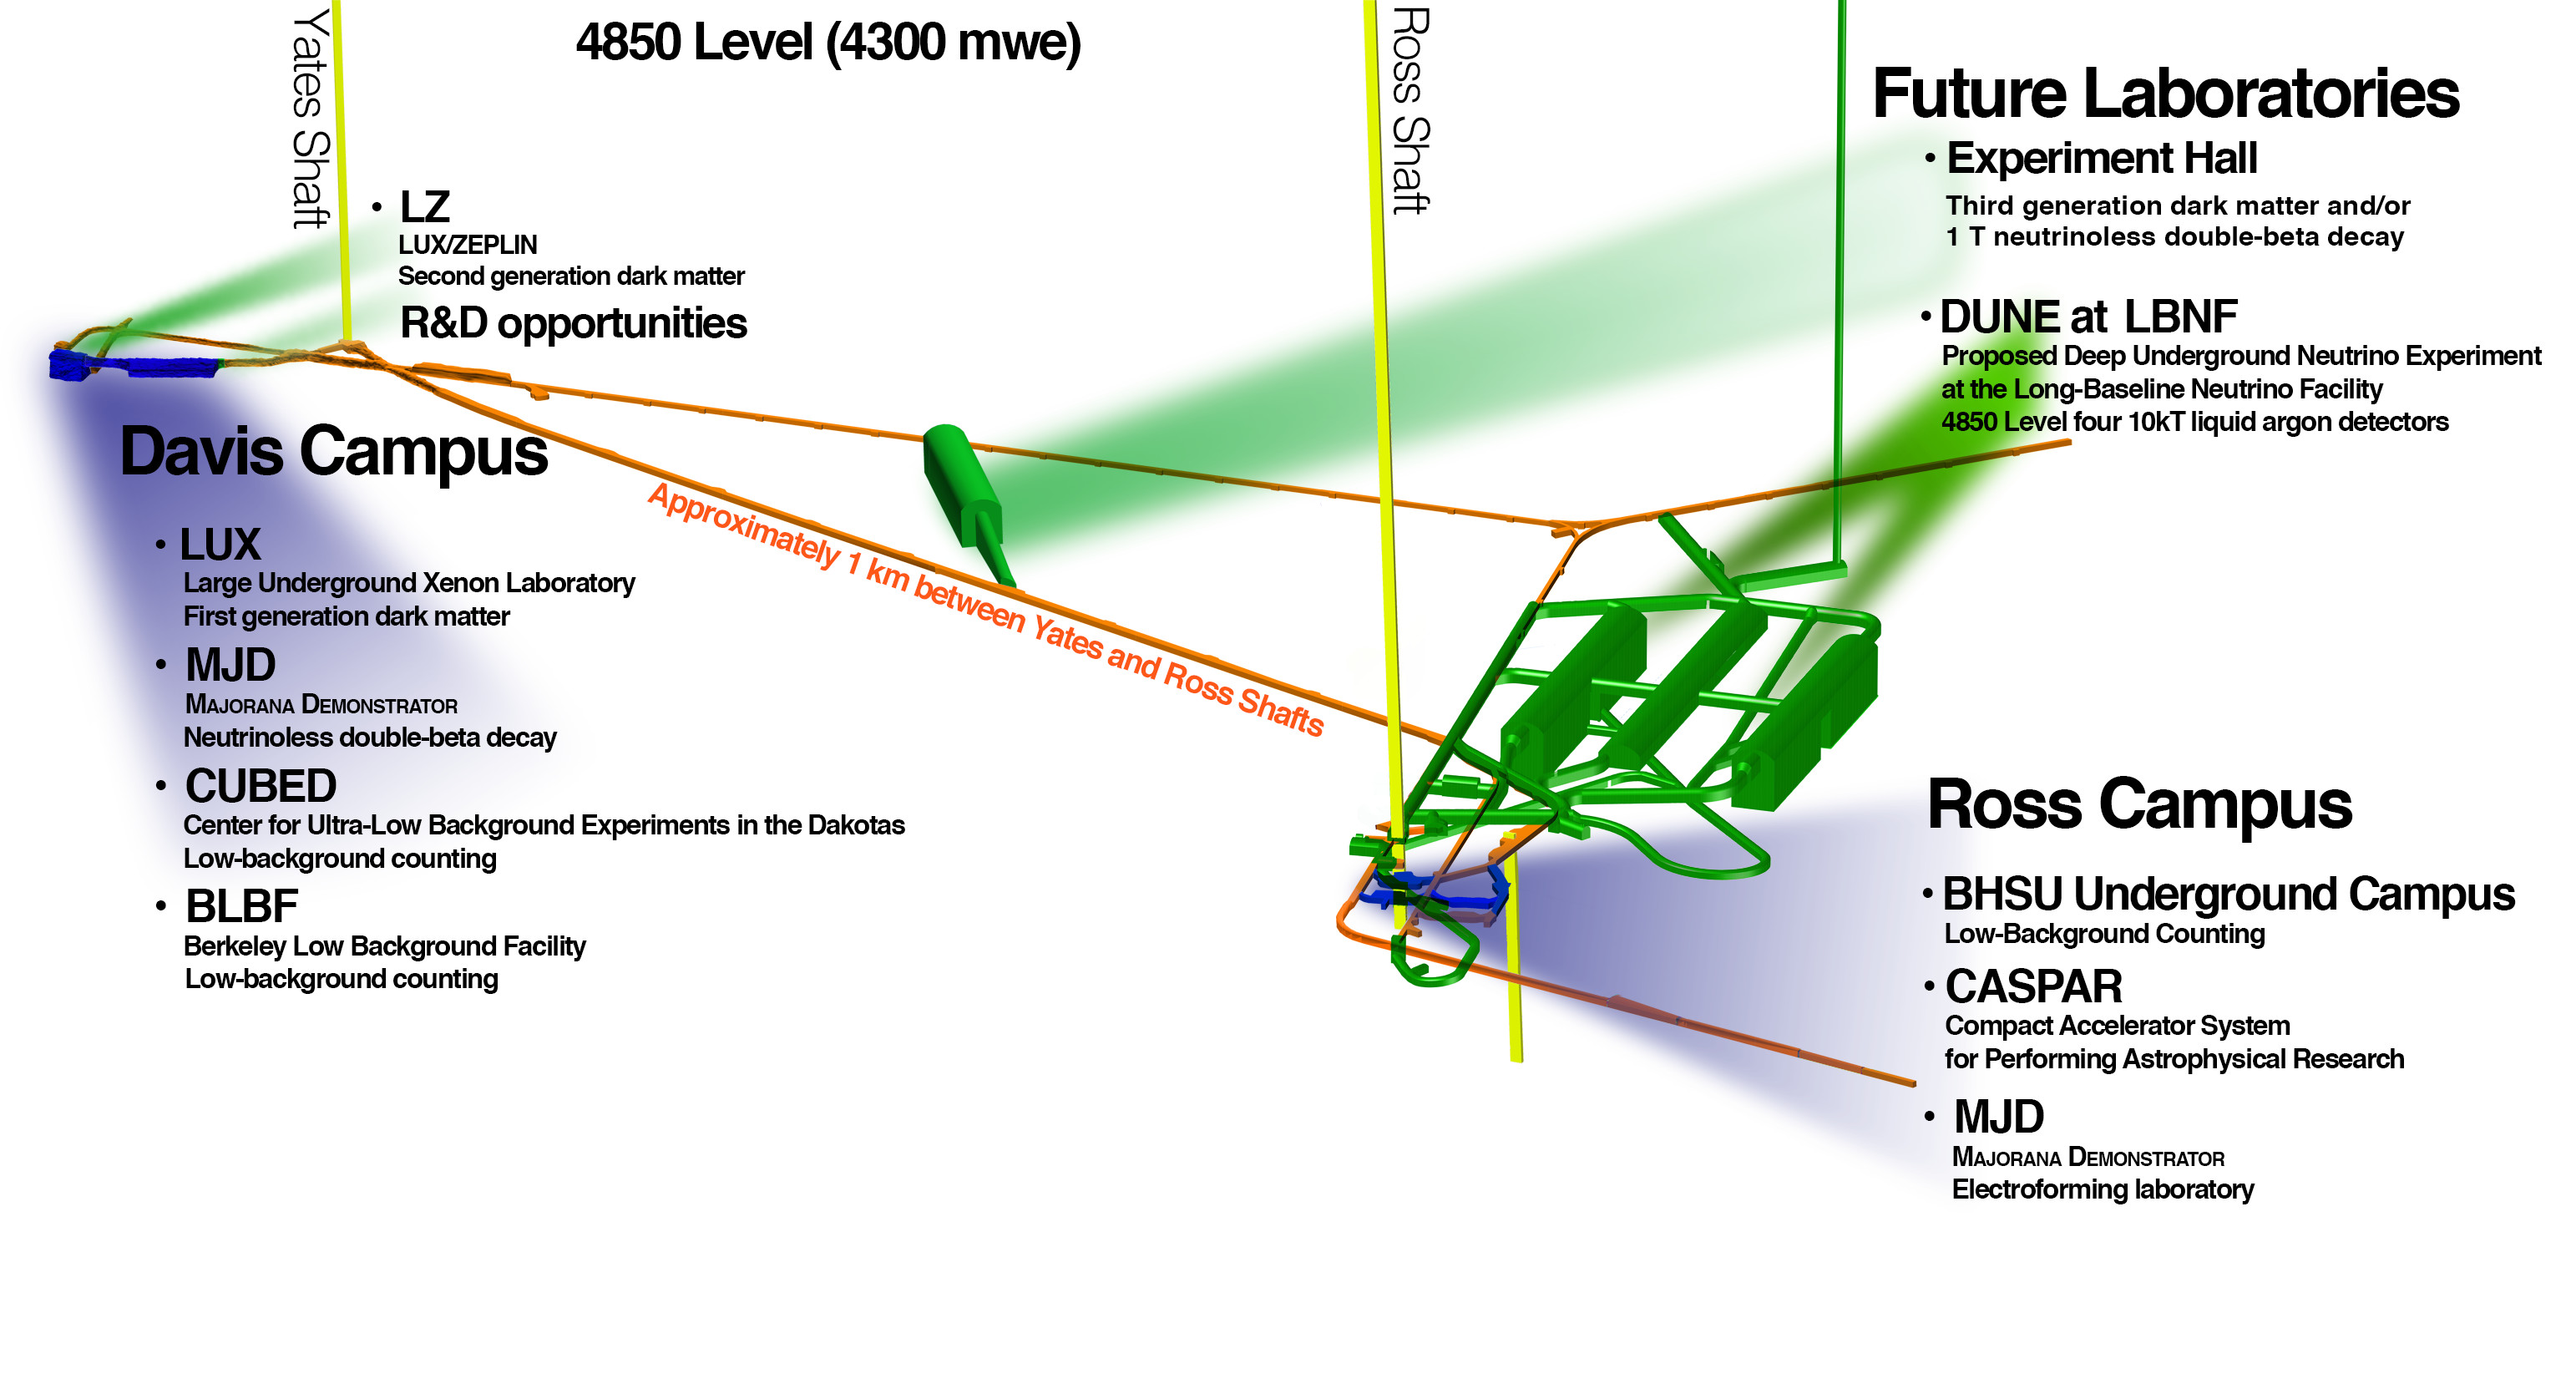
\includegraphics[width=0.8\textwidth]{underground-cavern-layout}
\end{cdrfigure}


%%%%%%%%%%%%%%%%%%%%%%%%%%%%%%%%%%
\section{Introduction to the Far Site Conventional Facilities}
\label{sec:fs-facil-cf}

This PDR presents the scope and necessary steps required to develop the LBNF Far Site Conventional Facilities (FSCF) at SURF. The key element of the FSCF is the underground space required to install and support the operations of the multi-module DUNE far detector. An overview of the 4850L at SURF where the underground facilities will be developed is shown in \ref{fig:underground-cavern-layout}.


While the SURF site already meets many requirements from the geological, scientific and engineering standpoint, significant work is required to provide adequate space and the infrastructure support needed for the experiment's installation and operation. The present and future state of the site, evaluation and assessments of the facilities and the associated provisioning of infrastructure such as power, water, plumbing, ventilation, etc., are described in this report. Also described are the safety measures and planned steps to develop the surface and underground structures. 

The scope of the FSCF includes design and construction for facilities on the surface and underground at SURF. The underground conventional facilities include new excavated spaces at the 4850L for the detector, utility spaces for experimental equipment, utility spaces for facility equipment, drifts for access, as well as construction-required spaces. Underground infrastructure provided by FSCF for the experiment includes power to experimental equipment, cooling systems and cyberinfrastructure. Underground infrastructure necessary for the facility includes domestic (potable) water, industrial water for process and fire suppression, fire detection and alarm, normal and standby power systems, a sump pump drainage system for native and leak water around the detector, water drainage to the facility-wide pump discharge system, and cyberinfrastructure for communications and security. In addition to providing new spaces and infrastructure underground, FSCF enlarges and provides infrastructure in some existing spaces for use, such as the access drifts from the Ross Shaft to the new caverns. New piping is provided in the shaft for cryogens (gas argon transfer line and nitrogen compressor suction and discharge lines) and water as well as power conduits and cyberinfrastructure.

As it exists today, SURF has many surface buildings and utilities, some of which will be utilized for LBNF. The scope of the above ground FSCF includes only that work necessary for LBNF, and not for the general rehabilitation of buildings on the site, which remains the responsibility of SURF. Electrical substations and distribution will be upgraded to increase power and provide standby capability for life safety. Additional surface scope includes remodeling of an existing building for both office space and to house an experiment/facility control room, and a new building to support cryogen transfer from the surface to the underground near the existing Ross Shaft. To reduce risk of failure of essential but aging support equipment during the construction and installation period, several SURF infrastructure-reliability activities are included as early activities in LBNF. These include completion of the Ross Shaft rehabilitation, rebuilding of hoist motors, and replacement of the Oro Hondo fan; if not addressed, failure of any of this aging infrastructure could limit or stop access to the underground.

This PDR is supported by a Design Report from the independent engineering firm, ARUP\cite{arup:fscf100pdr}.

%%%%%%%%%%%%%%%%%%%%%%%%%%%%%%%%%%%%%%%%%%%%%%%%%%%%%%%%%%%%%%%%%%%
\section{Structure of this Report}
\label{sec:pdr-volumes-fscf}

The scope of this Preliminary Design Report (PDR) is limited to the LBNF Far Site Conventional Facilities (FSCF); the cryogenics infrastructure is not included.
\begin{enumerate}
\item This chapter provides a short introduction to LBNF, DUNE and the FSCF.
\item Chapter~\ref{ch:intro-pm} summarizes the management structure for LBNF.
\item Chapter~\ref{ch:fscf-site-cond} describes the existing site conditions at SURF. 
\item Chapter~\ref{ch:fscf-surf-facil} describes the existing and planned surface buildings that will support the DUNE far detector, planned for installation at the 4850L of SURF.
\item Chapter~\ref{ch:fscf-excav} discusses the planned underground excavation. 
\item Chapter~\ref{ch:fscf-und-infra} describes the underground infrastructure that will directly interface to the DUNE far detector modules.
\end{enumerate}


